\section{Definition}
Channel decoding in NAVIC, the Indian Regional Navigation Satellite System, involves the process of error correction and retrieval of the original data transmitted over the satellite link. The channel decoding scheme used in NAVIC is based on a convolutional coding technique known as Rate 1/2 Convolutional Code with Viterbi decoding.
\subsection{Process}
Here is a high-level description of the channel decoding process in NAVIC:
\begin{figure}[h!]
	\centering
	%\subimport{table/}{table1.tex}
	

\tikzset{every picture/.style={line width=0.75pt}} %set default line width to 0.75pt        

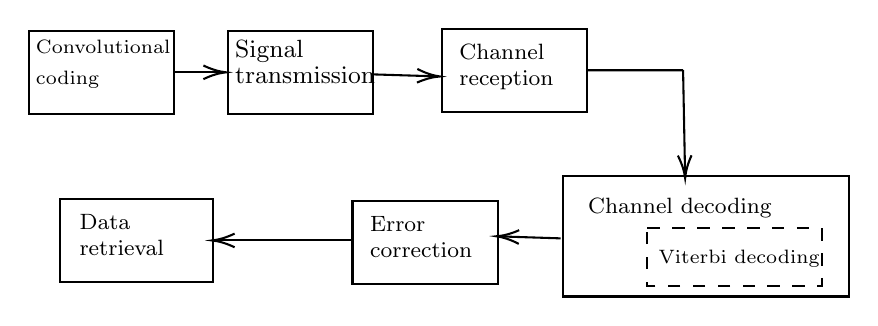
\begin{tikzpicture}[x=0.75pt,y=0.75pt,yscale=-1,xscale=1]
%uncomment if require: \path (0,300); %set diagram left start at 0, and has height of 300

%Shape: Rectangle [id:dp5040039695529985] 
\draw   (24,91) -- (94,91) -- (94,131) -- (24,131) -- cycle ;
%Straight Lines [id:da6707039679717985] 
\draw    (94.09,111.01) -- (117.09,111.01) ;
\draw [shift={(119.09,111.01)}, rotate = 180] [color={rgb, 255:red, 0; green, 0; blue, 0 }  ][line width=0.75]    (10.93,-3.29) .. controls (6.95,-1.4) and (3.31,-0.3) .. (0,0) .. controls (3.31,0.3) and (6.95,1.4) .. (10.93,3.29)   ;
%Shape: Rectangle [id:dp6676087786831228] 
\draw   (120,91) -- (190,91) -- (190,131) -- (120,131) -- cycle ;
%Shape: Rectangle [id:dp12552727666705787] 
\draw   (223,90) -- (293,90) -- (293,130) -- (223,130) -- cycle ;
%Shape: Rectangle [id:dp041785178904101716] 
\draw   (281.27,161.01) -- (419.27,161.01) -- (419.27,219.01) -- (281.27,219.01) -- cycle ;
%Shape: Rectangle [id:dp3930533301018766] 
\draw   (180,173) -- (250,173) -- (250,213) -- (180,213) -- cycle ;
%Shape: Rectangle [id:dp6457667866806436] 
\draw   (39.09,172) -- (113,172) -- (113,212) -- (39.09,212) -- cycle ;
%Straight Lines [id:da408023078866502] 
\draw    (190.09,112.01) -- (220.09,112.94) ;
\draw [shift={(222.09,113.01)}, rotate = 181.79] [color={rgb, 255:red, 0; green, 0; blue, 0 }  ][line width=0.75]    (10.93,-3.29) .. controls (6.95,-1.4) and (3.31,-0.3) .. (0,0) .. controls (3.31,0.3) and (6.95,1.4) .. (10.93,3.29)   ;
%Straight Lines [id:da20565488006754173] 
\draw    (339.27,110.01) -- (340.23,160.01) ;
\draw [shift={(340.27,162.01)}, rotate = 268.9] [color={rgb, 255:red, 0; green, 0; blue, 0 }  ][line width=0.75]    (10.93,-3.29) .. controls (6.95,-1.4) and (3.31,-0.3) .. (0,0) .. controls (3.31,0.3) and (6.95,1.4) .. (10.93,3.29)   ;
%Straight Lines [id:da606104691567432] 
\draw    (293,110) -- (339.27,110.01) ;
%Straight Lines [id:da9255999705919356] 
\draw    (280.27,191.01) -- (251.27,190.07) ;
\draw [shift={(249.27,190.01)}, rotate = 1.85] [color={rgb, 255:red, 0; green, 0; blue, 0 }  ][line width=0.75]    (10.93,-3.29) .. controls (6.95,-1.4) and (3.31,-0.3) .. (0,0) .. controls (3.31,0.3) and (6.95,1.4) .. (10.93,3.29)   ;
%Straight Lines [id:da848136557718163] 
\draw    (180.27,192.01) -- (114.27,192.01) ;
\draw [shift={(112.27,192.01)}, rotate = 360] [color={rgb, 255:red, 0; green, 0; blue, 0 }  ][line width=0.75]    (10.93,-3.29) .. controls (6.95,-1.4) and (3.31,-0.3) .. (0,0) .. controls (3.31,0.3) and (6.95,1.4) .. (10.93,3.29)   ;
%Shape: Rectangle [id:dp6659957800064993] 
\draw  [dash pattern={on 4.5pt off 4.5pt}] (322.09,186.01) -- (406,186.01) -- (406,214) -- (322.09,214) -- cycle ;

% Text Node
\draw (26,94) node [anchor=north west][inner sep=0.75pt]  [font=\small] [align=left] {{\scriptsize Convolutional}\\{\scriptsize coding}};
% Text Node
\draw (122,94) node [anchor=north west][inner sep=0.75pt]  [font=\footnotesize] [align=left] {{\small Signal }\\{\small transmission}};
% Text Node
\draw (230,96) node [anchor=north west][inner sep=0.75pt]  [font=\footnotesize] [align=left] {Channel \\reception};
% Text Node
\draw (326,195) node [anchor=north west][inner sep=0.75pt]  [font=\scriptsize] [align=left] {Viterbi decoding};
% Text Node
\draw (292,170) node [anchor=north west][inner sep=0.75pt]  [font=\footnotesize] [align=left] {Channel decoding};
% Text Node
\draw (187,179) node [anchor=north west][inner sep=0.75pt]  [font=\footnotesize] [align=left] {Error \\correction};
% Text Node
\draw (47,178) node [anchor=north west][inner sep=0.75pt]  [font=\footnotesize] [align=left] {Data\\retrieval};


\end{tikzpicture}


	\caption{The Block Level Architecture in Channel Decoding}
	\label{figs:decoderBlock}
	\end{figure}


\subsection{Convolutional Code Representation:}

The convolutional code is represented as a state diagram or trellis, where each state represents a unique history of the encoded bits.
The trellis consists of nodes and branches. Nodes correspond to states, and branches represent transitions between states.
Each branch is labeled with the input bit and the encoded output bits associated with the transition.

\subsection{Branch Metrics:}
At each time step, the Viterbi algorithm calculates branch metrics, which quantify the similarity between the received signal and the expected signal for each branch.
The branch metric is typically based on a distance measure, such as Hamming distance or Euclidean distance, between the received signal and the expected signal.
Let's denote the received signal at time step t as r(t) and the expected signal for a particular branch as c(t). The branch metric B(t) for that branch at time step t is computed as the distance between r(t) and c(t).

\subsection{Path Metrics:}
The Viterbi algorithm computes a path metric for each state at each time step, which represents the accumulated likelihood of reaching that state along a particular path.
The path metric is typically computed as the minimum (or maximum, depending on the metric used) of the sum of the previous path metric and the branch metric.
Let's denote the path metric for state i at time step t as P(i, t). The path metric for state i at time step t is computed as:
\begin{center}
P(i, t) = min{P(j, t-1) + B(t)}, where j is the previous state connected to state i.
\end{center}

\subsection{Survivor Paths:}
Along with the path metrics, the Viterbi algorithm keeps track of survivor paths, which represent the most likely paths leading to each state at each time step.
The survivor paths are determined based on the branch with the smallest (or largest, depending on the metric used) branch metric leading to each state.
The survivor paths help in traceback, as they indicate the most likely sequence of states leading to the current state.

\subsection{Traceback:}
Once the decoding reaches the end of the received signal, a traceback process is performed to determine the final decoded sequence.
Starting from the state with the highest path metric at the last time step, the algorithm traces back through the trellis by following the survivor paths.
The traceback process continues until reaching the starting state at the first time step, yielding the decoded sequence of transmitted bits.

\subsection{Decoding Output:}
The traceback process generates the final decoded output, which should ideally match the original transmitted data.
The decoded output undergoes error correction, such as using error-correcting codes like Reed-Solomon, to further enhance the reliability of the decoded sequence.

The Viterbi algorithm is an iterative process that calculates and updates the path metrics and survivor paths at each time step. It efficiently explores all possible paths through the trellis and selects the most likely path. This results in the recovery of the transmitted data even in the presence of noise and errors.

Let's solve the above mentioned step by step.
\begin{align}
Received\; signal : 
r = [0, 1, 1, 0, 0, 1, 1]\\
Generator\; polynomials :
G1 = 1 + D^2 + D^3 = 1 + D^2 + D^3\\
G2 = 1 + D + D^3 = 1 + D + D^3
\end{align}
We'll perform the Viterbi decoding process and calculate the path metrics and survivor paths.

Initialize path metrics and survivor paths:
\begin{align}
P[0, 0] = P[1, 0] = 0\\
S[0, 0] = S[1, 0] = []
\end{align}
Calculate branch metrics and update path metrics and survivor paths at each time step:\\
Time step t = 1:
\begin{align}
B[0, 1] = Hamming\; distance(r[1], 00) = 1\\
B[1, 1] = Hamming\; distance(r[1], 11) = 2\\
P[0, 1] = min(P[0, 0] + B[0, 1], P[1, 0] + B[1, 1]) = min(0 + 1, 0 + 2) = 1\\
P[1, 1] = min(P[0, 0] + B[0, 1], P[1, 0] + B[1, 1]) = min(0 + 1, 0 + 2) = 1\\
S[0, 1] = S[i_{min}, 0] + (0 or 1) = S[0, 0] + 0 = [0]\\
S[1, 1] = S[i_{min}, 0] + (0 or 1) = S[0, 0] + 0 = [0]
\end{align}
Time step t = 2:
\begin{align}
B[0, 2] = Hamming\; distance(r[2], 00) = 1\\
B[1, 2] = Hamming\; distance(r[2], 11) = 2\\
P[0, 2] = min(P[0, 1] + B[0, 2], P[1, 1] + B[1, 2]) = min(1 + 1, 1 + 2) = 2\\
P[1, 2] = min(P[0, 1] + B[0, 2], P[1, 1] + B[1, 2]) = min(1 + 1, 1 + 2) = 2\\
S[0, 2] = S[i_{min}, 1] + (0 or 1) = S[0, 1] + 0 = [0, 0]\\
S[1, 2] = S[i_{min}, 1] + (0 or 1) = S[0, 1] + 0 = [0, 0]
\end{align}
Time step t = 3 (continued):
\begin{align}
B[0, 3] = Hamming\; distance(r[3], 00) = 1\\
B[1, 3] = Hamming\; distance(r[3], 11) = 2\\
P[0, 3] = min(P[0, 2] + B[0, 3], P[1, 2] + B[1, 3]) = min(2 + 1, 2 + 2) = 3\\
P[1, 3] = min(P[0, 2] + B[0, 3], P[1, 2] + B[1, 3]) = min(2 + 1, 2 + 2) = 3\\
S[0, 3] = S[i_{min}, 2] + (0 or 1) = S[0, 2] + 0 = [0, 0, 0]\\
S[1, 3] = S[i_{min}, 2] + (0 or 1) = S[0, 2] + 0 = [0, 0, 0]
\end{align}
Time steps t = 4, 5, 6 (similar calculations as above).

Perform traceback:
\begin{center}
Identify 
$i_{max}$ = argmax(P[i, N-1]) = argmax(P[i, 6]) = argmax(P[0, 6], P[1, 6])
\end{center}
In this case,
\begin{center}
$i_{max}$ = 0 (as P[0, 6] = 5 and P[1, 6] = 4)
\end{center}
Start traceback from $i_{max}$ = 0, following the survivor paths backward.

Traceback:
\begin{align}
t = 6: S[0, 6] = [0, 0, 0]\\
t = 5: S[0, 5] = [0, 0]\\
t = 4: S[0, 4] = [0]\\
t = 3: S[0, 3] = [0, 0, 0]\\
t = 2: S[0, 2] = [0, 0]\\
t = 1: S[0, 1] = [0]\\
t = 0: S[0, 0] = []
\end{align}
The traceback process yields the decoded sequence: [0, 0, 0, 0, 0, 0, 0].

Therefore, the Viterbi decoding of the received signal [0, 1, 1, 0, 0, 1, 1] with the given generator polynomials G1 and G2 yields the decoded sequence [0, 0, 0, 0, 0, 0, 0].
\section{Software}
\begin{center}
 \begin{lstlisting}
Below python code realizes the above construction :
https://github.com/sivaparvathi-tungala/Channel-Decoding/blob/main/codes/decode.py
 \end{lstlisting}
\end{center}
